

The complex refractive index ($m$) describes the optical properties of the dust and is given by:
\begin{equation}
 m(\lambda) = n(\lambda) + ik(\lambda),
\end{equation}
\noindent where $n$ and $k$ are the real and imaginary parts of the refractive index, respectively \citep{Zhang2023}. 



For each filling factor and grain size in the distribution, \texttt{DSHARP} calculates several optical properties. These include the mass absorption and scattering coefficients, \kabs and \kscaNS, respectively. These coefficients describe how efficiently a material absorbs and scatters light. The resulting quantities are averaged over the grain-size distribution and are used to calculate additional parameters described below. 


Scattering can have a bias towards the forward direction, which is accounted for using $g$, the forward-scattering parameter defined by the expectation value of $\cos\Theta$ \citep{dsharp_code}. The scattering angle ($\Theta$) is the angle between the original direction and the new direction after it becomes polarized \citep{Zhang2023}. The parameter $g$ is used to calculate an effective scattering opacity, which is calculated by:
\begin{equation}
    \kscaeffEQ = (1-g)\kscaEQ.
\end{equation}
 




Figure \ref{fig: Kataoka2015Figure1Recreation} shows a replication of Figure 1 from \cite{Kataoka_2015}. This figure shows the absorption and scattering mass capacities, in units of \cmsq per gram, as a function of observing wavelength for maximum grain sizes of \amax = 1 \micron and 100 \micronNS. For the smaller dust grains (red lines, \amax = 1 \micronNS), the absorption opacity is much greater than the scattering opacity. For the larger dust grain (blue lines, \amax = 100 \micronNS), the scattering opacity is greater than the absorption opacity over approximately 0.1-2 mm. Therefore, at the observing wavelengths in this project, larger grains are more efficient at scattering than smaller grains. At the shorter and longer wavelength bounds, however, the scattering and absorption opacities are relatively similar.

\add{how the figure changes for different porosities}



% ----------------------------------------------
\begin{figure}[htbp]
  \centering
  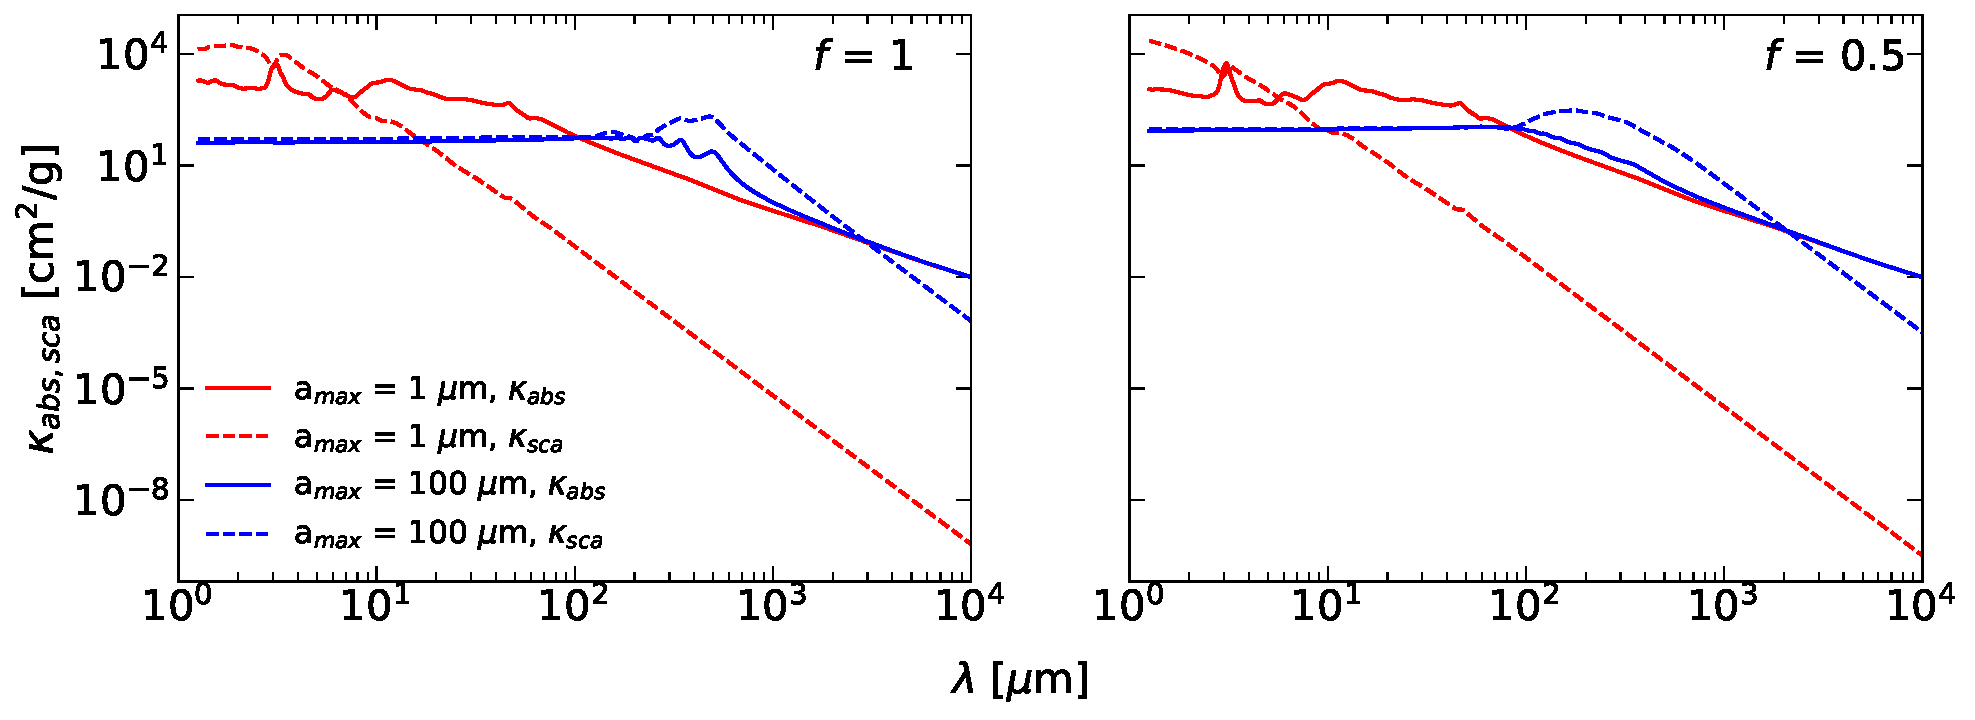
\includegraphics[width=0.6\textwidth]{WRITEUP_AND_IMAGES/IMAGES/WRITEUP/DustModels/Kataoka2015Fig1_grid.pdf}
  \caption{Absorption and scattering mass opacities as a function of observing wavelength for grain sizes of 1\micron and 100 \micron for compact (left) and porous (right) grains. Recreation of Figure 1 from \cite{Kataoka_2015}. \code{add plot, f = 1 left, f = 0.5 right} \intextref{update after plot change}  \code{change this to smoothed data?}}
  \label{fig: Kataoka2015Figure1Recreation}
\end{figure}
% ----------------------------------------------
\begin{figure}[htbp]
  \centering
  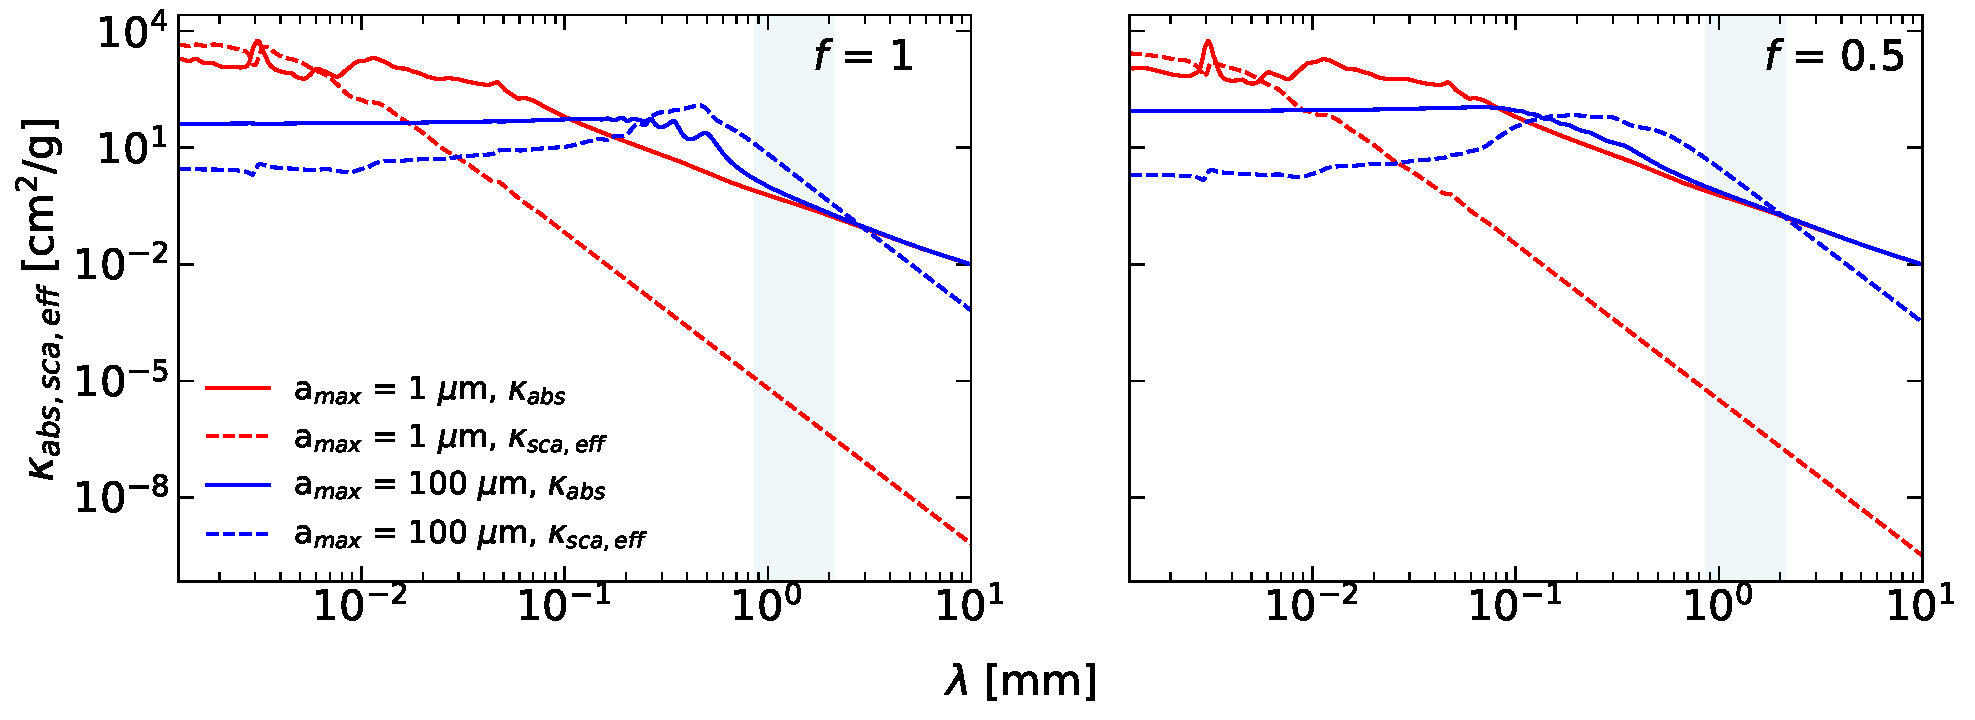
\includegraphics[width=0.6\textwidth]{WRITEUP_AND_IMAGES/IMAGES/WRITEUP/DustModels/Kataoka2015Fig1_grid_eff.pdf}
  \caption{\add{caption}}
  \label{fig: Kataoka2015Figure1Recreation_eff}
\end{figure}
% ----------------------------------------------



%



An additional quantity is the single scattering albedo, which describes the fraction of the original light that is removed by scattering rather than absorption. The standard and effective albedo are defined as \citep{Zhang2023}:
\begin{equation}
    \omega = \frac{\kscaEQ}{\kabsEQ + \kscaEQ}, \quad 
    \weffEQ = \frac{\kscaeffEQ}{\kabsEQ + \kscaeffEQ}.
    \label{eq: omega}
\end{equation}


\add{something about which one we are using and why, refer to paper Daniel sent}
% \question{As far as I know, glitterin is using $\omega$ and not $\omega_{eff}$, meaning when I present the results for spherical vs irregular, I'm comparing $P\omega_{eff}$ vs $P\omega$. I am not entirely sure how to get the $g$ factor I need to calculate $\omega_{eff}$ with gitterin. I only switched to $\omega_{eff}$ because of \cite{Zhang2023}. Should I switch the spherical back to just $\omega$ so they are comparing the same thing?} \SC{A: I would contact Daniel and ask if this is important.  How much of a difference is omega versus omega\_eff?}
